\documentclass[10pt]{beamer}

\usetheme[progressbar=frametitle, block=fill]{metropolis}
\RequirePackage{amsmath,amssymb,amsthm,graphicx,mathrsfs,url,slashed,subcaption}
\usepackage{appendixnumberbeamer}

\usepackage{booktabs}
\usepackage[scale=2]{ccicons}

\usepackage{pgfplots}
\usepgfplotslibrary{dateplot}

\newcommand{\NN}{\mathbf{N}}
\newcommand{\ZZ}{\mathbf{Z}}
\newcommand{\QQ}{\mathbf{Q}}
\newcommand{\RR}{\mathbf{R}}
\newcommand{\CC}{\mathbf{C}}
\newcommand{\DD}{\mathbf{D}}
\newcommand{\PP}{\mathbf P}
\newcommand{\MM}{\mathbf M}
\newcommand{\II}{\mathbf I}
\newcommand{\Hyp}{\mathbf H}
\newcommand{\Sph}{\mathbf S}
\newcommand{\Group}{\mathbf G}
\newcommand{\GL}{\mathbf{GL}}
\newcommand{\Orth}{\mathbf{O}}
\newcommand{\SpOrth}{\mathbf{SO}}
\newcommand{\Ball}{\mathbf{B}}

\newcommand*\dif{\mathop{}\!\mathrm{d}}
\newcommand{\dfn}[1]{\emph{#1}\index{#1}}

\newcommand{\Teich}{\mathrm{Teich}}
\newcommand{\normal}{\mathbf n}

\newcommand{\dist}{\mathrm{dist}}
\newcommand{\id}{\mathrm{id}}
\newcommand{\Lip}{\mathrm{Lip}}
\newcommand{\loc}{\mathrm{loc}}
\newcommand{\cpt}{\mathrm{cpt}}


\newcommand{\Two}{\mathrm{I\!I}}


\newtheorem{proposition}{Proposition}
\newtheorem{philosophy}{Philosophy}
\newtheorem{question}{Question}
\newtheorem{conjecture}{Conjecture}


\usepackage{xspace}
\newcommand{\themename}{\textbf{\textsc{metropolis}}\xspace}

\title{Convex duality between calibrations and laminations, and $L^\infty$ and $BV$ variational problems}
% \subtitle{A modern beamer theme}
% \date{\today}
\date{???, 2025}
\author{Aidan Backus}
\institute{Brown University}
% \titlegraphic{\hfill\includegraphics[height=1.5cm]{logo.pdf}}

\begin{document}

\maketitle

% \begin{frame}{Table of contents}
%   \setbeamertemplate{section in toc}[sections numbered]
%   \tableofcontents%[hideallsubsections]
% \end{frame}

\begin{frame}{Philosophy}
    \centering
    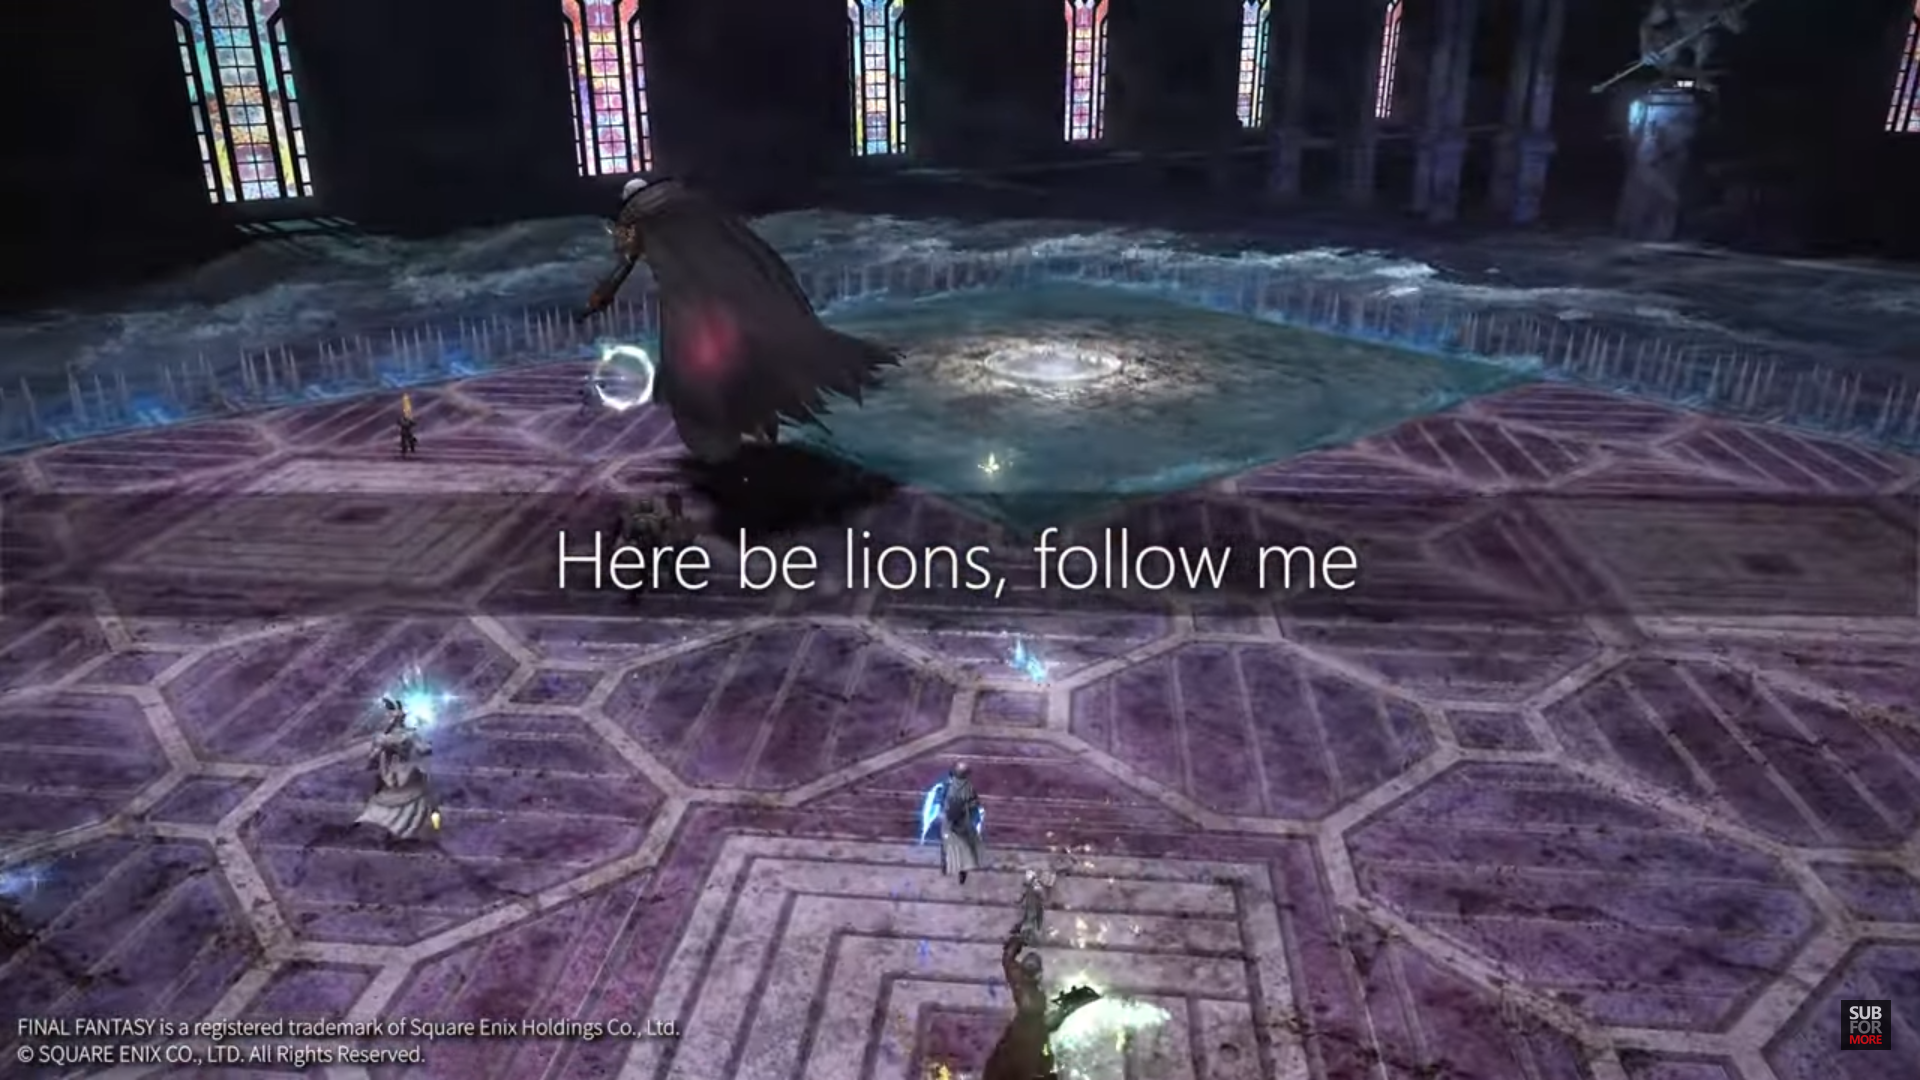
\includegraphics[width=\textwidth]{hic_svnt_leones}
\end{frame}

\begin{frame}{de Giorgi lemma}
    \centering
    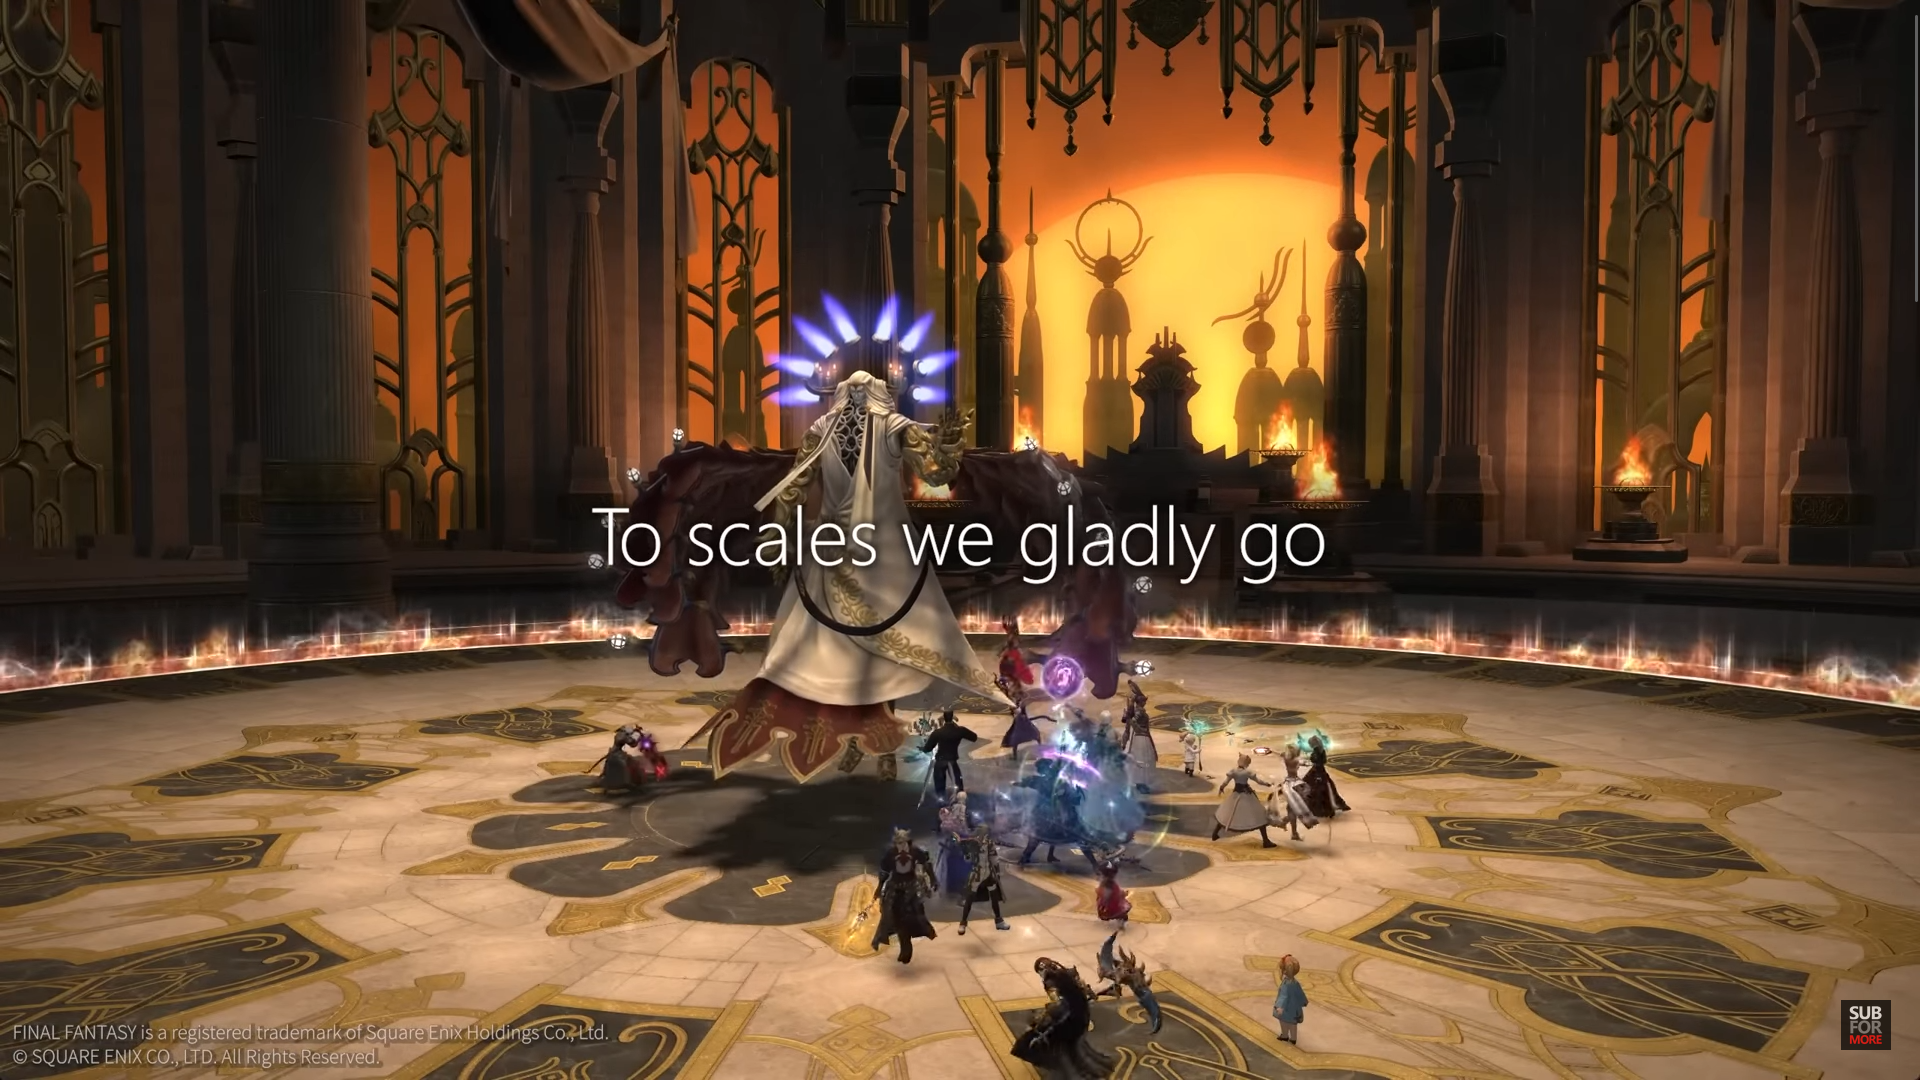
\includegraphics[width=\textwidth]{to_scales}
\end{frame}

\begin{frame}{The operator norm}
    \centering
    
\includegraphics[width=0.8\textwidth]{operator_norm}
\end{frame}

\end{document}
